
\section{基于GDB内核调试}
在软件开发过程中,调试是不可避免的。一个程序往往不会一开始就按照程序员预期的方式运行, 对操作系统这样的复杂巨系统而言尤其如此。本节主要讲解调试软件GDB的使用方法。
\subsection{认识GDB}
GNU调试器(英语:GNU Debugger,缩写:GDB),是GNU软件系统中的标准调试器,此外GDB也是个具有移携性的调试器,经过移携需求的调修与重新编译,如今许多的类UNIX操作系统上都可以使用GDB,而现有GDB所能支持调试的编程语言有C、C++、Pascal以及FORTRAN。

\textbf{为什么需要GDB}

当程序出现错误时,开发者需要快速地找出错误的原因,并修复它们。很多人会倾向于使用"人工静态分析"(也就是目测法和冥想法)解决Bug。

然而,程序的运行时状态往往非常复杂,有时很难在代码中准确地定位错误。 具体来说, 目测的以下缺点导致开发者往往会百思不得其解进而无功而返:

\textbf{1.无法检测运行时问题:}代码静态分析只能检测静态代码问题,例如语法错误、类型错误等,它无法检测代码的运行时问题。例如,它无法检测到由于代码在特定环境下执行而引起的问题,如内存泄漏、死锁等。

\textbf{2.误报和漏报:}静态分析可能会误会遗漏问题。例如,可能会将某些无害的代码标记为错误,或者忽略某些实际上是错误的代码。这可能会导致开发人员浪费时间和精力来调查错误的根本原因。

\textbf{3.对高质量代码的依赖:}代码静态分析需要高质量的代码才能进行准确的分析。如果代码质量不好,例如缺乏注释、变量名不规范、代码冗余等,那么静态分析可能会产生误报或漏报。

\textbf{4.难以发现复杂的问题:}静态分析工具通常使用各种分析技术来分析代码,但这些技术很难发现复杂的问题,例如多线程问题、分布式系统问题等。这些问题通常需要动态调试或其他更高级的技术来解决。

同样, 也有人会尝试插入LOG打印部分状态, 但是这种方法除了费时费力, 且暴露状态不够精确的问题之外, 在OS中, 某些LOG会产生系统状态的改变, 进而影响结果, 导致debug失败。

这时候,调试工具就显得非常重要了。调试工具可以帮助开发者在运行时监视程序的状态,跟踪代码的执行流程,查看变量的值,以及定位错误的位置。 这正是GDB的用途。

GDB 最初由Richard Stallman在他的GNU Emacs 系统稳定后于1986年编写,并设计作为他的GNU系统的一部分。GDB是根据GNU通用公共许可证(GPL)发布的免费软件。它是在Berkeley Unix发行版附带的DBX调试器之后建模的。从1990 年到 1993 年,它由John Gilmore维护。现在由自由软件基金会任命的 GDB 指导委员会维护。

GDB允许用户查看一个程序在执行时“内部”的执行过程—,或者查看程序在崩溃时的内部状态。这些被调试的程序可以与 GDB 在同一台机器上(本地)、另一台机器(远程)或模拟器上执行。GDB 可以在大多数流行的 UNIX 和 Microsoft Windows 变体以及 Mac OS X 上运行。具体而言,目前 GDB 支持以下程序:Ada、Assembly、C、C++、D、Fortran、Go、Objective-C、OpenCL、Modula-2、Pascal、Rust 等。

GDB 默认只有命令行接口(CLI)可用,而不具备较能亲合上手、直觉操作的图形用户界面(GUI),不过此一弱处也已经有几个前端程序为其补强,例如DDD、GDBtk/Insight (页面存档备份,存于互联网档案馆)以及Emacs中的“GUD 模式”等,有了这些补强后,GDB在功效使用的便利性上就能够与“集成发展环境中的调试功效使用”相接近。

\textbf{GDB的启动}

显然, 启动gdb有不同的方法, 在终端中输入gdb是最简单的, 但NPUcore在RISC-V上构建, 因此不能直接使用本机的gdb(除非你使用一台RISC-V64计算机),因此我们推荐安装并使用gdb-multiarch(这里需要Ubuntu环境):
\begin{lstlisting}[language={Rust}, label={code:forktest},
	caption={forktest.rs}]
	$ sudo apt-get install gdb-multiarch
	# 然后启动:
	$ gdb-multiarch
\end{lstlisting}

注意, 这里实际上有"工作目录"的概念, 也就是你的当前目录实际上最好在项目或者源代码的路径上, 否则会需要手工加载源代码路径(方法见下文)。
\subsection{基于GDB的内核调试}
\textbf{QEMU虚拟机的相关命令}

介绍GDB为什么要先介绍虚拟机呢?因为正是QEMU与GDB合作, 才给了我们方便地进行大部分系统软件调试的机会。

作为一款全虚拟化虚拟机, QEMU能彻底模拟CPU的内部状态, 包括寄存器和其他部分, 因此很适合进行调试。

具体来说, QEMU配合GDB提供了单步执行、断点调试、内存监视、寄存器查看等。

用户可以使用调试功能逐步执行代码,查看每一步的运行结果和寄存器状态,同时还可以设置断点,方便定位问题所在。

利用QEMU提供的远程调试功能,允许用户在另一台计算机上通过网络连接到QEMU的调试接口进行调试。这个功能可以方便地在不同的计算机之间进行协作开发和调试。

这里我们只介绍本地的远程调试。

为了方便, 在os文件夹中, 使用下列make命令直接进行gdb调试:
\begin{lstlisting}[language={Rust}, label={code:forktest},
	caption={forktest.rs}]
	make gdb
\end{lstlisting}
其后端执行实际命令是:
\begin{lstlisting}[language={Rust}, label={code:forktest},
	caption={forktest.rs}]
	gdb:
	@qemu-system-riscv64 -machine virt -nographic -bios $(BOOTLOADER) -device loader,\
	file=target/riscv64gc-unknown-none-elf/debug/os,addr=0x80200000 -drive \
	file=$(U_FAT32),if=none,format=raw,id=x0 \
	-device virtio-blk-device,drive=x0,bus=virtio-mmio-bus.0 -smp threads=$(CORE_NUM) -S -s
\end{lstlisting}  
和do-run的内容相比,
\begin{lstlisting}[language={Rust}, label={code:forktest},
	caption={forktest.rs}]
	do-run:
	@qemu-system-riscv64 \
	-machine virt \
	-nographic \
	-bios $(BOOTLOADER) \
	-device loader,file=$(KERNEL_BIN),addr=$(KERNEL_ENTRY_PA) \
	-drive file=$(U_FAT32),if=none,format=raw,id=x0 \
	-device virtio-blk-device,drive=x0,bus=virtio-mmio-bus.0\
	-smp threads=$(CORE_NUM)
\end{lstlisting}  
不难发现最主要的差别在于后面多出的"-S -s"。 前面的S代表STOP, 意思是设置完虚拟机直接挂起, 停止一切执行, 直到接收到外部的continue信息为止.

第二个小写s等价于"-gdb tcp::1234",指的是开启远程调试,其在localhost(本机)的1234端口侦听GDB的信号, 等待连接。 然后, 就是我们的下一个工具GDB的任务和工作范畴了。

\begin{figure}[htb]
\centering
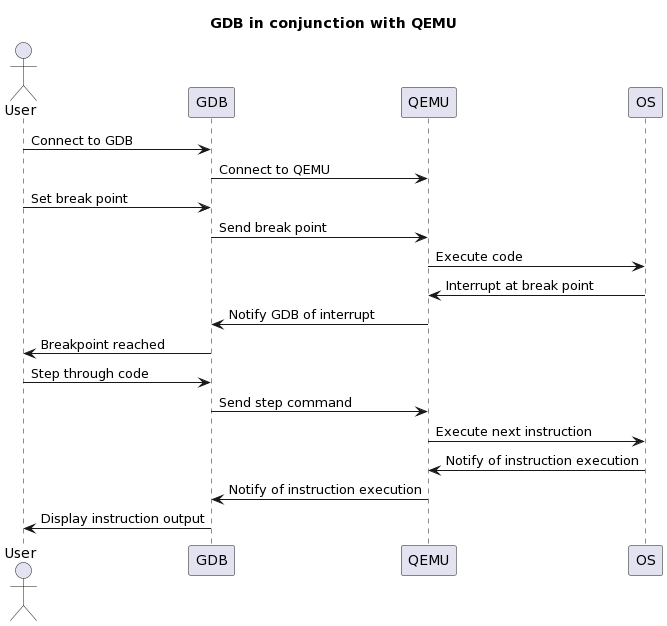
\includegraphics[width=\textwidth]{figures/02-02-GDB联调QEMU的逻辑流程.png}
\caption{
	GDB联调QEMU的逻辑流程
}
\label{fig:GDB联调QEMU的逻辑流程}
\end{figure}

\textbf{历史}
在GDB的命令行(和各种IDE的GDB控制台)中, 使用上下左右(或者Alt-P之类的自定义按键)可以直接显示之前的命令, 这和Bash是一致的。

但和Bash不同的是, 其重复执行上一条命令可以通过直接在不进行任何输入的时候敲回车实现:

\begin{lstlisting}[language={Rust}, label={code:forktest},
	caption={forktest.rs}]
	(gdb) stepi
	(gdb) (然后这里敲回车)
\end{lstlisting} 

这时候就前进了两条指令。但这个功能也会导致有时候多按了一下回车结果重复执行了某些只应当被执行一次的指令, 因此也要注意使用的场景。
\textbf{补全}

GDB命令的确数量庞大且内容复杂, 但是但作为一款老牌软件, GDB自然也有解决方案。一方面, GDB自己提供了强大的命令补全功能, 能像在Bash中一样TAB补全,例如如下所示的键盘输入:输入b然后按下TAB键, 会补全为break, 其他的, 如寄存器名称等往往也可以在有了部分提示前缀后进行补全。 因此不需要每次都键入完整的命令。

\textbf{辅助}

另一方面, 多数的IDE和编辑器都有辅助GDB的功能, 例如在某一行代码旁边点击行号附近的位置, 会出现一个圆点, 表示加入断点。

另外, 如果你需要重复某个命令多遍, 并不需要一直按着鼠标或者键盘回车键, 只需要在命令后面插入重复次数即可:

\begin{lstlisting}[language={Rust}, label={code:forktest},
	caption={forktest.rs}]
	(gdb) stepi 4
\end{lstlisting}

这里就前进了4条指令。

\textbf{常见命令}

进入gdb, 会看到"(gdb)"提示可以输入命令(有时候无法输入)。

如果在VSCode中使用, 还需要在之前加上exec

\begin{lstlisting}[language={Rust}, label={code:forktest},
	caption={forktest.rs}]
	exec gdb <...>
\end{lstlisting}

\textbf{设定命令}
(1) 连接

按照之前的方法启动QEMU后, GDB要通过下列命令连接本地的QEMU。

\begin{lstlisting}[language={Rust}, label={code:forktest},
	caption={forktest.rs}]
	target remote :1234
	
	<div align=center><img src="./pic/1.2/remote.png" style="zoom:100%"></div> 
	
	如果你之前指定了自定义的端口, 需要将1234换成其他的端口号。同时, 冒号之前实际上省略了localhost(也就是本机的“网址”), 如果你将来有自定义的地址或者网址, 也可以在前面补上。
\end{lstlisting}

(2) 加载调试信息

\begin{lstlisting}[language={Rust}, label={code:forktest},
	caption={forktest.rs}]
	(1)file
	在开始调试之前, 你首先需要加载调试信息。
	file target/riscv64gc-unknown-none-elf/debug/os
	从而加载os文件作为符号文件。请注意, 使用release版本的文件(在make命令中加入“MODE=release”得到)往往不带有任何的调试信息, 不适合用于debug, 但也不尽然: 你可以对着汇编语言调试。 当然, 就算使用了带有符号文件的版本,这种体验你总会遇到的, 因为操作系统总是要涉及某些底层。
	这里加载的是操作系统的符号, 那如果某些过程经过用户程序(作为一个操作系统, 你总会遇到这种问题), 如何添加用户程序的代码?这就要用到一下一个命令了。
	如果先连接QEMU后加载二进制文件, 就会出现上面的"A program is being debugged already."提示,当然这并不影响使用。
	
	$add-symbol-file
	
	$ add-symbol-file bash
	
\end{lstlisting}

如果你的当前工作文件夹中具有bash文件, 就可以直接添加, 否则需要自行前往特定的。 显然, 上面两个命令的顺序可以修改, 但注意, file只能有一个, symbol-file却可以有很多, 且符号文件指代的不一定是带有符号部分的可执行文件, 也可能是纯粹的符号文件(考虑到其和主题无关,这里的内容我们不拓展,读者可以进一步查找资料)。 这时候可以info files显示所有已经添加的符号和二进制文件

\begin{figure}[htb]
\centering
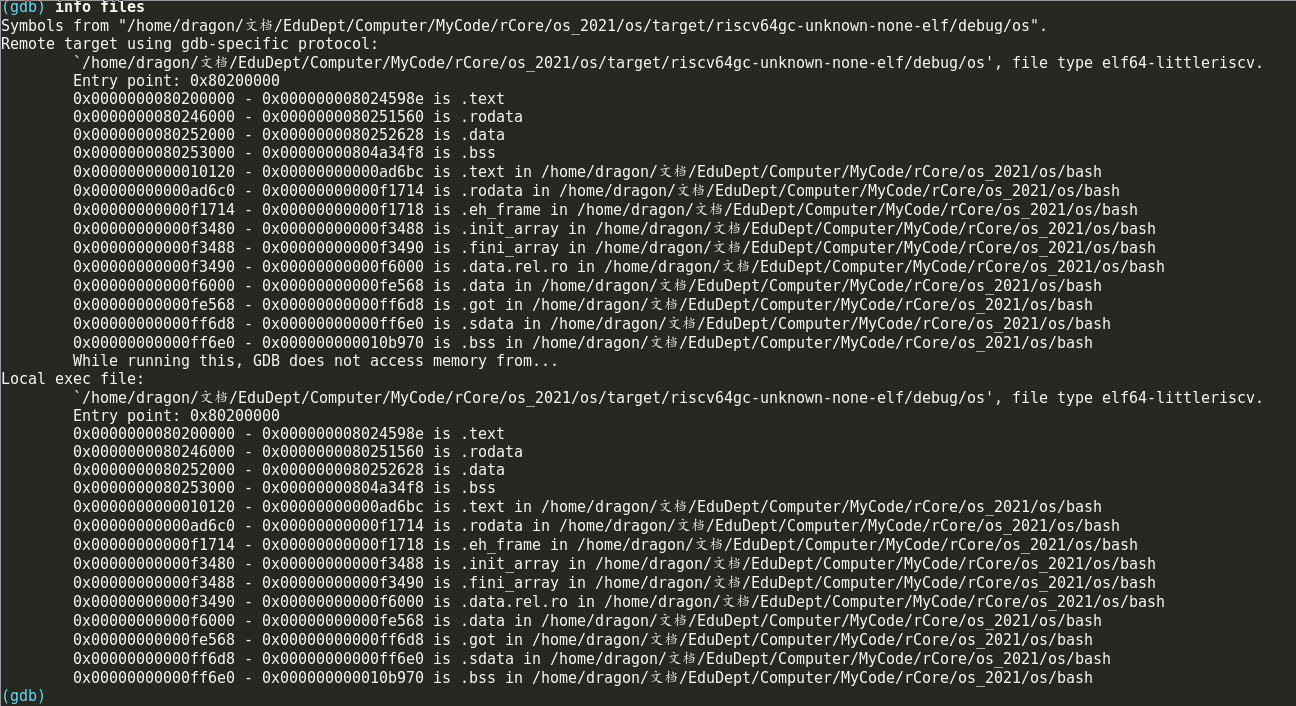
\includegraphics[width=\textwidth]{figures/02-02-info files.png}
\caption{
	info files
}
\label{fig:info files}
\end{figure}

\begin{lstlisting}[language={Rust}, label={code:forktest},
	caption={forktest.rs}]
	(1)directory
	设置完符号文件, 接着需要设置源代码目录, 这样在IDE/GDB中可以自动跳转到函数代码所在处。
	$dir ~/Downloads/SW/Bash/bash-5.1.16/
	$dir ~/Downloads/SW/Bash/bash-5.1.16/lib/sh/
	注意, 这里需要你将bash的源代码先提前下载好到某个目录, 并将上面的这个路径替换成正确的目录。
	最终得到:
	Source directories searched: /home/dragon/Downloads/SW/Bash/bash-5.1.16/lib/sh:/home/dragon/Downloads/SW/Bash/bash-5.1.16:$cdir:$cwd
	另外,部分的软件目录结构复杂, 这时候需要手动用上述命令添加。
	(2)break
	break用于设置断点。可以通过断点中断程序的执行并让你进入调试模式。
	一般常见的断点设定方式有:文件:行号格式和函数(方法)格式
	例如:(基于特定版本, 你的具体地址与行号可能不同)
	$(gdb) b src/main.rs:50
	Breakpoint 1 at 0x900000000004f158: file src/main.rs, line 59.
	$(gdb) b rust_main
	Breakpoint 2 at 0x900000000004f198: file src/main.rs, line 66.
	
	注意! 函数名方法有时候要指定域, 格式类似os::rust_main;
	如果要删除断点, 则可以
	$delete 1
	跟上断点号即可。
	(3)set
	set可以是多种的, 最典型的是让pc强制移动到某个位置, 例如:
	$set $pc=0x0
	回到最开始的执行点。 当然, 你也可以用它对别的地址/变量进行强行赋值。
	
\end{lstlisting}

\textbf{执行流}

(1)continue
很显然, GDB有两种状态, 停止和执行, 只有在停止的时候, 我们才能对其中的数据进行查看和修改, 对自己的命令进行调整,而continue正是从停止到执行的切换工具。

continue会继续执行程序直到遇到下一个断点或程序结束。 这条命令往往用于target remote :1234后继续执行。

例如, 我们一开始执行make gdb只有:

\begin{lstlisting}[language={Rust}, label={code:forktest},
	caption={forktest1.rs}]
	$ make gdb
\end{lstlisting}

一个光标停在原地。

但是, 如果你在gdb中输入continue并回车, 虚拟机马上就会停止冻结,开始执行指令(直到撞到某个停止条件为止):

\begin{figure}[htb]
\centering
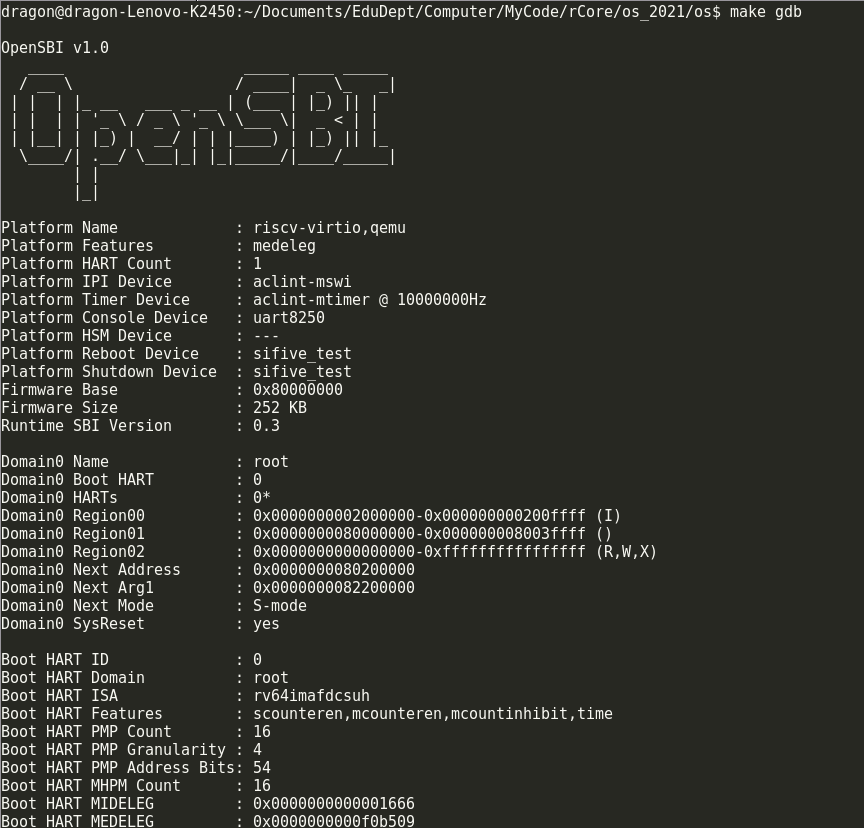
\includegraphics[width=\textwidth]{figures/02-02-设置断点.png}
\caption{
	设置断点
}
\label{fig:设置断点}
\end{figure}

此时, 命令就会停在之前设定的断点上
(2)暂停或终止运行

在终端和多数IDE中, 暂停执行流是通过gdb控制台(注意不是虚拟机的终端, 而是gdb的控制台)ctrl-C(同时按下Ctrl和C)实现的, 这可以让程序暂停在当前执行到的位置。

如果你之前在执行QEMU时没有加入“-S”选项, 那么你可以用这条命令立即暂停执行流(当然其具体停止位置难以保证。)

完成后debug后, 可以用quit退出。

(3)next,step和finish

stepi前进一条指令.

\begin{figure}[htb]
\centering
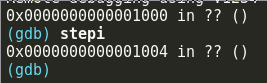
\includegraphics[width=\textwidth]{figures/02-02-stepi.png}
\caption{
	stepi
}
\label{fig:stepi}
\end{figure}

next可以单步执行程序,跳过函数调用,例如(中间省略几步continue和break):

\begin{figure}[htb]
\centering
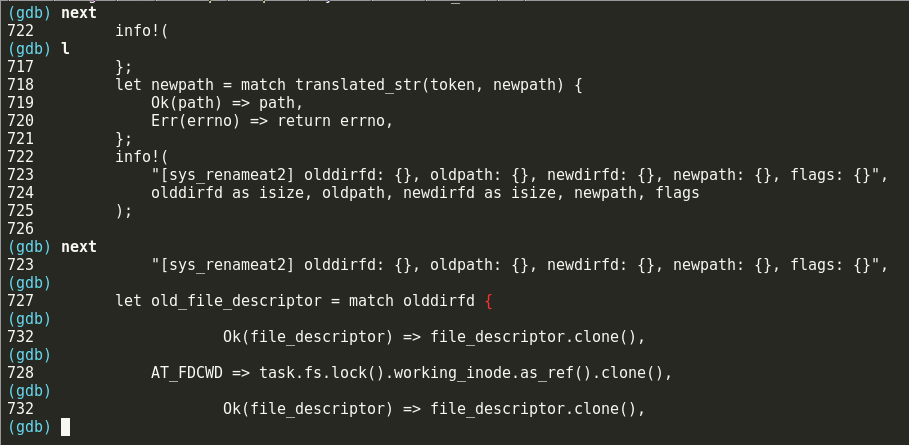
\includegraphics[width=\textwidth]{figures/02-02-next.png}
\caption{
	next
}
\label{fig:next}
\end{figure}

可以看到这里的几条函数都被跳过了。

step单步执行程序,进入函数调用(这里的执行流进入了函数调用):

\begin{figure}[htb]
\centering
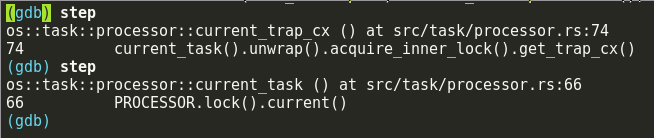
\includegraphics[width=\textwidth]{figures/02-02-step.png}
\caption{
	step
}
\label{fig:step}
\end{figure}

finish执行完当前函数并返回到调用函数, 然后又回到了之前的函数:

\begin{figure}[htb]
\centering
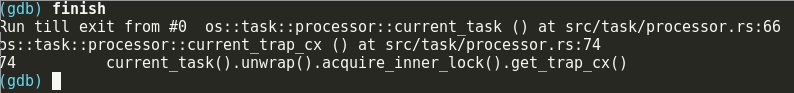
\includegraphics[width=\textwidth]{figures/02-02-finish.png}
\caption{
	finish
}
\label{fig:finish}
\end{figure}

\textbf{查看命令}

在停止状态下, 我们可以backtrace显示函数调用栈:

\begin{figure}[htb]
\centering
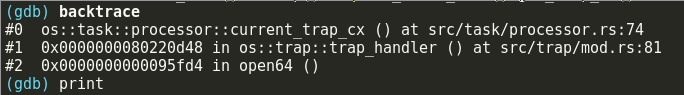
\includegraphics[width=\textwidth]{figures/02-02-backtrace.png}
\caption{
	backtrace
}
\label{fig:backtrace}
\end{figure}

或者print打印寄存器/变量/内存地址的值:

\begin{figure}[htb]
	\centering
	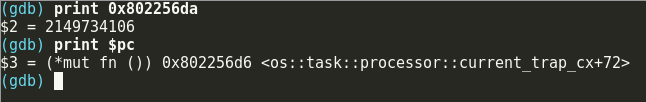
\includegraphics[width=\textwidth]{figures/02-02-print.png}
	\caption{
		print
	}
	\label{fig:print}
\end{figure}

如果觉得每次都打印很麻烦,可以用display每次停在断点处时自动打印某个变量的值。一旦不需要, 可以undisplay该号码取消(类似delete语法),如下列这段话打印附近前后各6条汇编代码(其他的变量也可以打印,语法类似)

\begin{lstlisting}[language={Rust}, label={code:forktest},
	caption={forktest1.rs}]
	display/12i $pc-6*4
\end{lstlisting}

\begin{figure}[htb]
\centering
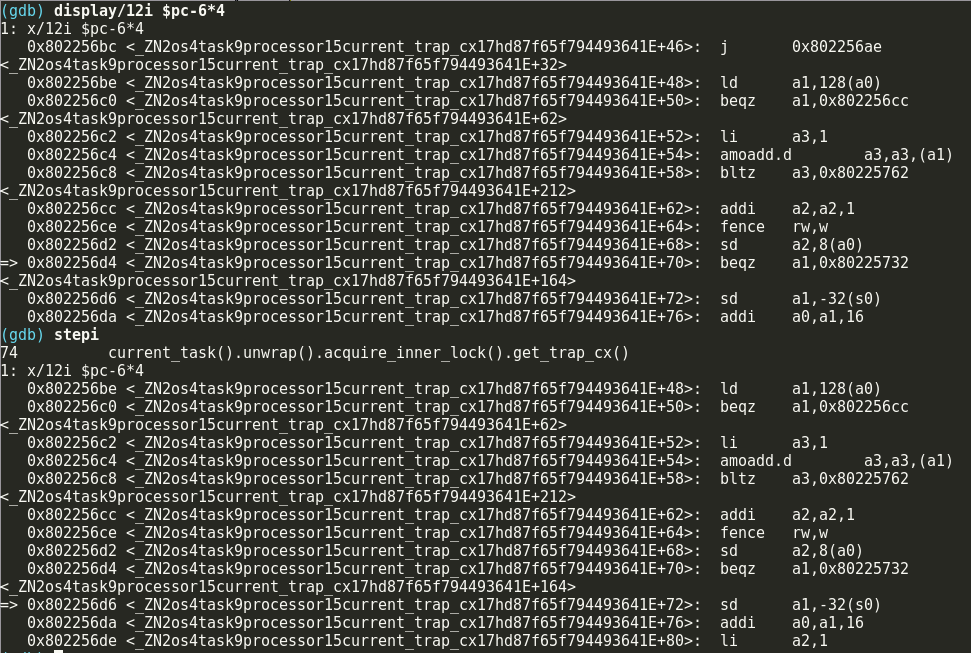
\includegraphics[width=\textwidth]{figures/02-02-display.png}
\caption{
	display
}
\label{fig:display}
\end{figure}

也可以info registers打印所有的寄存器

\begin{figure}[htb]
\centering
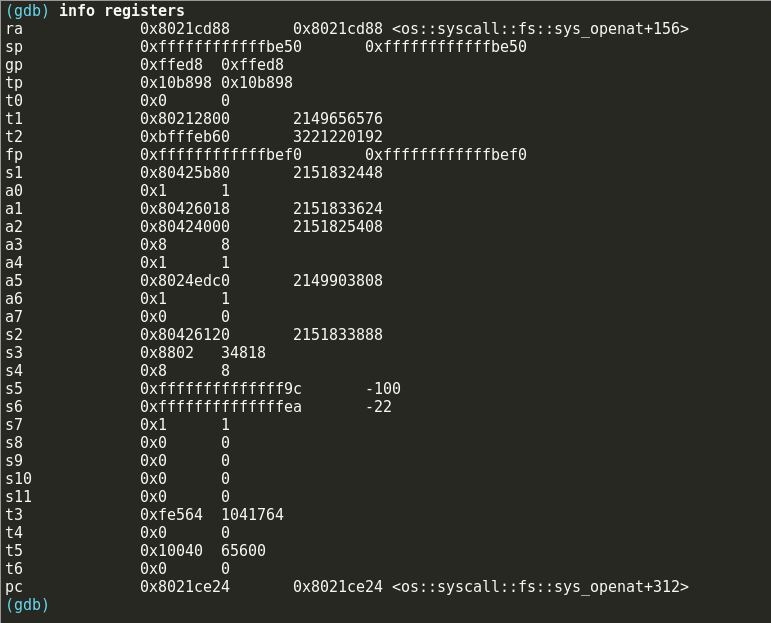
\includegraphics[width=\textwidth]{figures/02-02-info registers.png}
\caption{
	info registers
}
\label{fig:info registers}
\end{figure}

\textbf{自定义命令与脚本}

在使用GDB进行调试时,我们需要多次执行一些常见的指令。为了提高调试效率,我们可以使用define命令来定义自己的命令,简化重复操作。

下面我们来介绍如何定义一个自定义命令。首先,使用文本编辑器创建一个gdb脚本文件,例如mycommands.gdb。然后,在该文件中添加以下代码:

\begin{lstlisting}[language={Rust}, label={code:forktest},
	caption={forktest1.rs}]
	# 加载符号文件
	file target/riscv64gc-unknown-none-elf/debug/os
	add-symbol-file bash
	# 井号加入注释
	define mynext
	stepi
	info registers
	end
	# 添加bash的源代码
	dir 
\end{lstlisting}

这个自定义命令名为mynext,执行的操作包括执行下一条指令和显示所有寄存器的值。

接下来,启动GDB并加载定义的自定义命令。我们可以通过以下命令将mycommands.gdb文件加载到GDB中:

\begin{lstlisting}[language={Rust}, label={code:forktest},
	caption={forktest1.rs}]
	source mycommands.gdb
\end{lstlisting}

现在,我们可以在GDB中使用mynext命令来执行下一条指令并显示所有寄存器的值。只需在GDB提示符下输入“mynext”即可。

使用define自定义命令可以帮助我们快速地执行常见的调试操作,提高调试效率。 另外,其他的断点添加, 远程调试连接等命令也可以很方便地加入其中从而加速Debug过程。

在命令行下启动 GDB 并加载脚本时,可以使用 -x 或 –command 选项来指定要执行的脚本文件。该选项后跟要执行的脚本文件路径,如下所示:

\begin{lstlisting}[language={Rust}, label={code:forktest},
	caption={forktest1.rs}]
	# -x 选项指定了要执行的脚本文件路径,file_to_debug 则是要调试的目标程序的路径。
	gdb -x /path/to/script file_to_debug
	# 除了 -x 选项外,还可以使用 --init-command 选项指定要执行的初始化命令,该选项可以多次使用,每次指定一条命令,如下所示:
	gdb --init-command="set print pretty on" --init-command="set pagination off" file_to_debug
	# 上述命令中,--init-command 选项指定了要执行的初始化命令,可以多次使用,每次指定一条命令。
\end{lstlisting}


\subsection{git bisect——快速问题定位}
大家一定听过二分查找的算法, 如果我们发现某个Bug出现, 其实也可以通过二分查找定位到出错的版本。
git也自带了这个功能。使用git bisect, 我们可以在Git版本控制系统中进行二分查找,在版本历史中快速定位错误引入的位置。
\textbf{一般步骤}
我们以这些图文为例给出一个错误的处理
\begin{lstlisting}[language={Rust}, label={code:forktest},]
	$ git bisect start
	//运行 git bisect start 命令来启动一个二分查找会话。
	$ git bisect bad
	//用 git bisect bad 命令告诉 Git 当前版本存在问题。
	$ git bisect good HEAD~10
	//用 git bisect good 命令告诉 Git 一个知道没有问题的提交, 是这个提交的哈希值或分支名。git会给出估计的剩余步骤数
	Bisecting: 4 revisions left to test after this (roughly 2 steps)
	[f55d253527e3a72f730b06e6fbfe5e64f8594a27] fix: Change ELF related AuxV data alignment to repr(C), fixing the LPF.
	//Git 会自动切换到一个介于上述两个提交之间的提交,你需要在该提交上运行你的程序,检查问题是否存在。
	如果有问题,使用 git bisect bad 命令告诉 Git,否则使用 git bisect good 命令告诉 Git。
	你可以使用Git bisect run 切换提交后自动执行的命令(注意, git bisect run后仍然在原地, 这时候需要git bisect next才能进入下一个, 否则会冲突)
	Git 会根据你的反馈自动切换到下一个介于两个提交之间的提交,重复上述步骤,直到找到引入问题的提交。
	最后,使用 git bisect reset 命令退出二分查找会话。
\end{lstlisting}

\begin{figure}[htb]
	\centering
	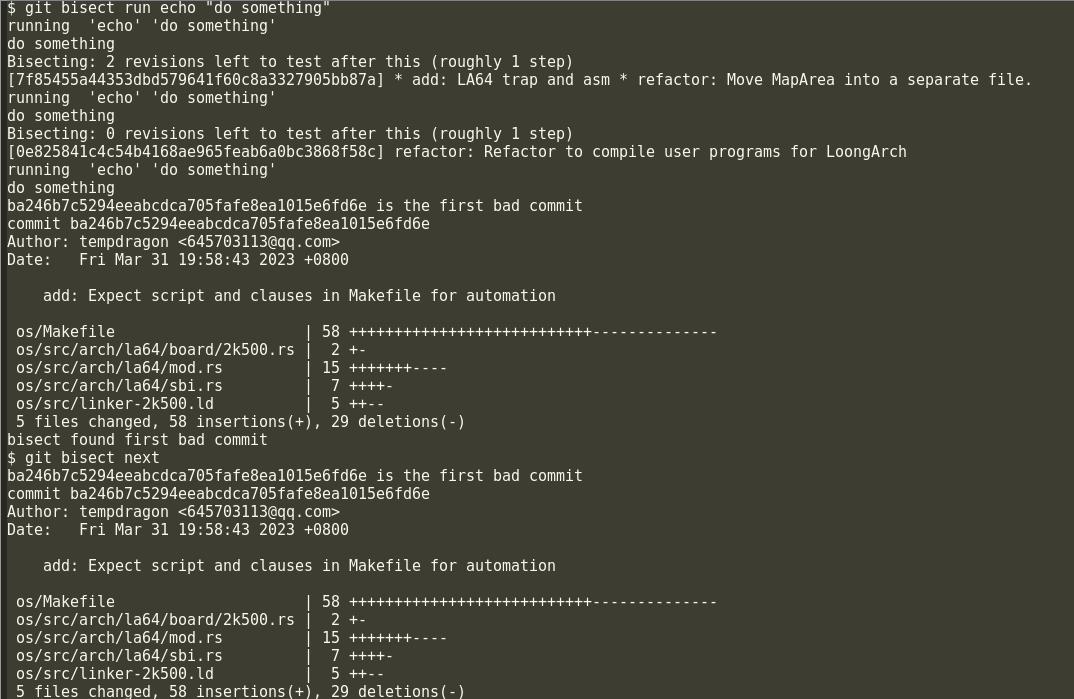
\includegraphics[width=\textwidth]{figures/02-02-运行实例.png}
	\caption{
		运行实例
	}
	\label{fig:运行实例}
\end{figure}
\textbf{log与冲突回撤}
如果发现某个提交被错误标记(比如bad被错误标记为good), 尝试
\begin{lstlisting}[language={Rust}, label={code:forktest},]
	git bisect bad
	你会得到以下错误:
	ba246b7c5294eeabcdca705fafe8ea1015e6fd6e was both good and bad
	
	$ git bisect log//导出日志:
	
	git bisect start
	# good: [ba246b7c5294eeabcdca705fafe8ea1015e6fd6e] add: Expect script and clauses in Makefile for automation
	git bisect good ba246b7c5294eeabcdca705fafe8ea1015e6fd6e
	# bad: [ba246b7c5294eeabcdca705fafe8ea1015e6fd6e] add: Expect script and clauses in Makefile for automation
	git bisect bad ba246b7c5294eeabcdca705fafe8ea1015e6fd6e
	//重定向到文件
	$ git bisect log > bis.log
	//考虑修改错误
	$ git bisect start
	会得到以下信息:
	# bad: [ba246b7c5294eeabcdca705fafe8ea1015e6fd6e] add: Expect script and clauses in Makefile for automation
	$ git bisect bad ba246b7c5294eeabcdca705fafe8ea1015e6fd6e
	
	$ git bisect replay bis.log
	//回复到之前的状态
\end{lstlisting}  
